\documentclass[compress]{beamer}
\usepackage[
    title={Parallel Matrix Multiplication},
    event={Progetto fine corso SCPA},
    author={MC, LF},
    longauthor={Matteo Conti, Luca Falasca},
    email={},
    institute={SCPA 2023-2024},
    longinstitute={Universita' degli Studi di Roma Tor Vergata},
]{unislides}
\usepackage{graphicx} % Required for inserting images
\usepackage{minted}
\usepackage{algorithm}
\usepackage{hyperref}
\usepackage{adjustbox}
\usepackage{svg}
\svgsetup{inkscapelatex=false}

\begin{document}

\begin{frame}[plain]
    \titlepage
\end{frame}

%---------------------INTRODUZIONE---------------------
\section{Introduzione}

\subsection{Descrizione del problema}
\begin{frame}{\secname \text{ }- \subsecname\ }
    Il progetto verte sull'implementazione di un nucleo di calcolo per effettuare il prodotto tra due matrici dense, definito come:
    \begin{Definition}
        \begin{equation}
            \label{eq:ce_ue}
            C = C + A\cdot B
        \end{equation}
    \end{Definition}
    dove $A$, $B$ e $C$ sono matrici di dimensioni $M\times K$, $K\times N$ ed $M\times N$ rispettivamente, in particolare verranno considerate:
    \begin{itemize}
        \item Matrici quadrate
        \item Matrici rettangolari con $M,N>>K$ con $K=\{32, 64, 128, 156\}$
    \end{itemize}
\end{frame}

\subsection{Obiettivi}
\begin{frame}{\secname \text{ }- \subsecname\ }
    Verranno analizzate le prestazioni di tre differenti implementazioni del prodotto, in particolare:
    \begin{columns}
        \column{0.5\textwidth}
            \begin{minipage}[b]{1\textwidth}
                \begin{itemize}
                    \item MPI, utilizzando il paradigma SIMD per la parallelizzazione su CPU
                    \item CUDA, sfruttando le potenzialità delle GPU per l'accelerazione computazionale
                    \item MPI+CUDA, cercando di combinare i vantaggi delle due precedenti versioni
                \end{itemize}
            \end{minipage}
        \column{0.5\textwidth}
            \begin{minipage}{1\textwidth}
                \begin{adjustbox}{margin=0cm 0cm 0cm 0.2cm, center} % left, bottom, right, top
                    
\includegraphics[width=0.5\textwidth]{resources/cpu_gpu.png}
                \end{adjustbox}
            \end{minipage}
    \end{columns}
\end{frame}

\subsection{Metriche di valutazione}
\begin{frame}{\secname \text{ }- \subsecname\ }
    Per valutare le prestazioni delle soluzioni sviluppate la metrica utilizzata sono i FLOPS, i quali sono definiti come:
    \begin{Definition}
        \begin{equation}
            FLOPS = \frac{2MNK}{exec\_time}
        \end{equation}
    \end{Definition}
    \begin{adjustbox}{margin=0cm 0cm 0cm 0.2cm, center} % left, bottom, right, top
        
\includegraphics[width=0.25\textwidth]{resources/performance_icon.png}
    \end{adjustbox}
\end{frame}

\subsection{Raccolta dei dati}
\begin{frame}{\secname \text{ }- \subsecname\ }
    I dati raccolti sono stati ottenuti eseguendo i vari nuclei di calcolo sul server di dipartimento il quale presenta le seguenti specifiche:
    \begin{columns}
        \column{0.5\textwidth}
            \begin{minipage}[b]{1\textwidth}
                \begin{itemize}
                    \item CPU: 2 x Intel Xeon Silver 4210
                    \item Memory: 64 GiB of RAM
                    \item GPU: Nvidia Quadro RTX 5000
                    \item CUDA version: 12.3
                    \item MPI version: 4.1
                \end{itemize}
            \end{minipage}
        \column{0.5\textwidth}
            \begin{minipage}{1\textwidth}
                \begin{adjustbox}{margin=0cm 0cm 0cm 0.6cm, center} % left, bottom, right, top
                    
\includegraphics[width=0.65\textwidth]{resources/pc.png}
                \end{adjustbox}
            \end{minipage}
    \end{columns}
\end{frame}

%---------------------MPI------------------------------
\section{MPI}

\begin{frame}{\secname}
    In questa sezione verranno presentate la versione dell'implementazione del prodotto tra matrici utilizzando le funzionalità offerte da MPI per la parallelizzazione su CPU, in particolare verranno affrontati tre aspetti:
    \vspace{0.5cm}
    \begin{columns}
        \column{0.5\textwidth}
            \begin{minipage}[b]{1\textwidth}
                \begin{itemize}
                    \item Distribuzione del carico
                    \item Riduzione del risultato
                    \item Implementazione del prodotto
                \end{itemize}
            \end{minipage}
            \column{0.5\textwidth}
                \begin{minipage}{1\textwidth}
                    \begin{adjustbox}{margin=0cm 0cm 0cm 0.3cm, center} % left, bottom, right, top
                        
\includegraphics[width=0.5\textwidth]{resources/parallel_icon.png}
                    \end{adjustbox}
                \end{minipage}
    \end{columns}
\end{frame}

\subsection{Distribuzione del carico}
\begin{frame}{\secname \text{ }- \subsecname\ (1)}
    Per la distribuzione del carico è stato utilizzato un approccio analogo a quello utilizzato dalla libreria ScaLAPACK, cioè la block cyclic distribution, questa tecnica permette di distribuire la matrice di partenza in modo da bilanciare il carico tra i processi in modo abbastanza ragionevole. La tecnica si basa su tre idee:
    \vspace{0.3cm}
    \begin{itemize}
        \item I processi vengono visti come una griglia $P_r \times P_c$
        \item La matrice viene divisa in blocchi di dimensione $B_r \times B_c$
        \item La griglia dei processi viene fatta scorrere in modo tumbling sui blocchi assegnando tali blocchi ai processi
    \end{itemize}
\end{frame}
\begin{frame}{\secname \text{ }- \subsecname\ (2)}
Le matrici A, B e C vengono distribuite come segue:
\begin{columns}
    \column{0.5\textwidth}
        \begin{minipage}[b]{1\textwidth}
            \begin{adjustbox}{margin=0cm 0cm 0.5cm 0cm, center} % left, bottom, right, top
                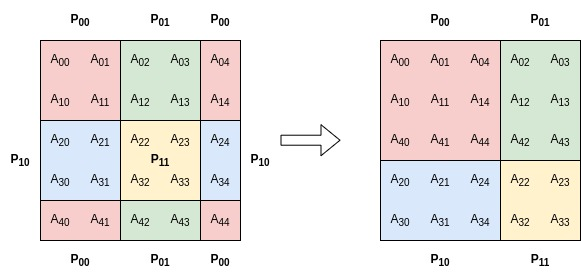
\includegraphics[width=0.95\textwidth]{resources/matrixA_2d_block_cyclic_distribution.jpg}
            \end{adjustbox}
        \end{minipage}
        \column{0.5\textwidth}
            \begin{minipage}{1\textwidth}
                \begin{adjustbox}{margin=0cm 0cm 0.5cm 0cm, center} % left, bottom, right, top
                    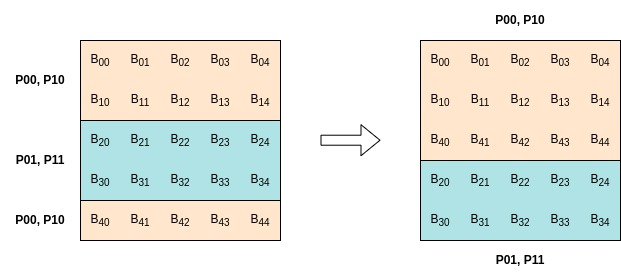
\includegraphics[width=1\textwidth]{resources/matrixB_row_block_cyclic_distribution.jpg}
                \end{adjustbox}
            \end{minipage}
    \end{columns}
    \begin{adjustbox}{margin=0cm 0cm 0.5cm 0.3cm, center} % left, bottom, right, top
        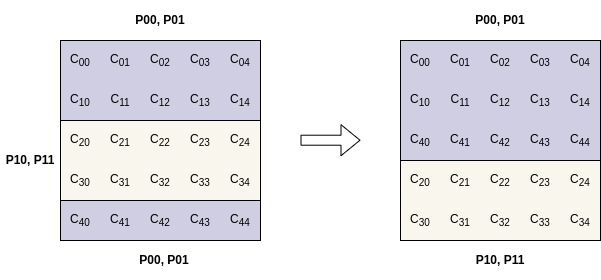
\includegraphics[width=0.5\textwidth]{resources/matrixC_row_block_cyclic_distribution.jpg}
    \end{adjustbox}
\end{frame}

\subsection{Riduzione del risultato}
\begin{frame}{\secname \text{ }- \subsecname\ }
    Dato che ogni riga di processi nella process grid partecipa alle stesse K righe del risultato, si è scelto di non effettuare la riduzione su un solo processo bensì di definire per ogni riga un \textit{row leader}. \\\\I leader effettuano la riduzione dei risultati parziali di tutti i processi nella loro riga e successivamente scriveranno su file il risultato senza interferire tra loro, in quanto scriveranno in punti diversi.
    \begin{adjustbox}{margin=0cm 0cm 0cm 0.3cm, center} % left, bottom, right, top
        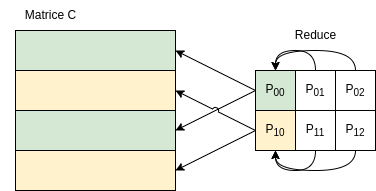
\includegraphics[width=0.5\textwidth]{resources/reduce.png}
    \end{adjustbox}
\end{frame}

\subsection{Implementazione del prodotto}
\begin{frame}{\secname \text{ }- \subsecname\ }
    L'effettiva implementazione del prodotto è stata realizzata in due versioni:
    \vspace{0.3cm}
    \begin{itemize}
        \item \textit{Naive}, implementazione semplice che non tiene conto di ottimizzazioni
        \item \textit{Column blocked}, implementazione più complessa che ottimizza l'utilizzo della cache
    \end{itemize}
    \begin{adjustbox}{margin=0cm 0cm 0cm 0.7cm, center} % left, bottom, right, top
        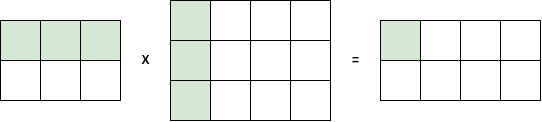
\includegraphics[width=0.7\textwidth]{resources/product_icon.png}
    \end{adjustbox}
\end{frame}

\subsubsection*{Naive}
\begin{frame}{\secname \text{ }- \subsecname\ \text{ }- \subsubsecname}
    Questa implementazione è composta da soli tre cicli che permettono di scorrere le matrici e costruire il risultato.
    \begin{adjustbox}{margin=0cm 0cm 0cm 0.5cm, center} % left, bottom, right, top
        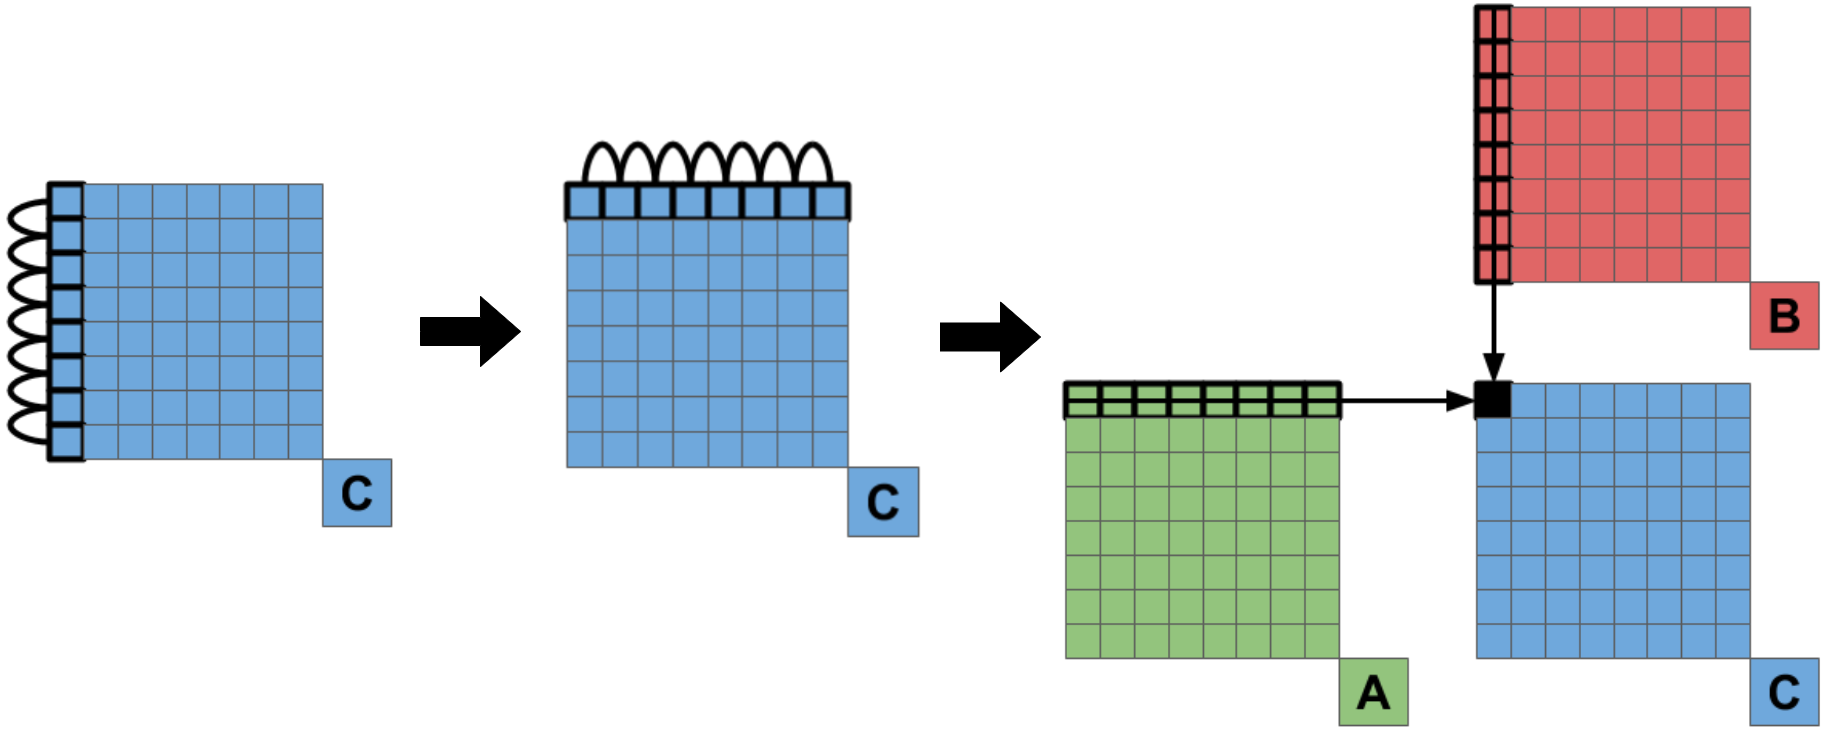
\includegraphics[width=0.95\textwidth]{resources/naive_icon.png}
    \end{adjustbox}    
\end{frame}

\subsubsection*{Column blocked}
\begin{frame}{\secname \text{ }- \subsecname\ \text{ }- \subsubsecname}
    Qui viene tenuto conto del fatto che quando si accede un elemento della matrice esso viene caricato in cache insieme ai 15 elementi successivi, è possibile quindi riorganizzare il processamento per sfruttare fenomeno.
    \begin{adjustbox}{margin=0cm 0cm 0cm 0.7cm, center} % left, bottom, right, top
        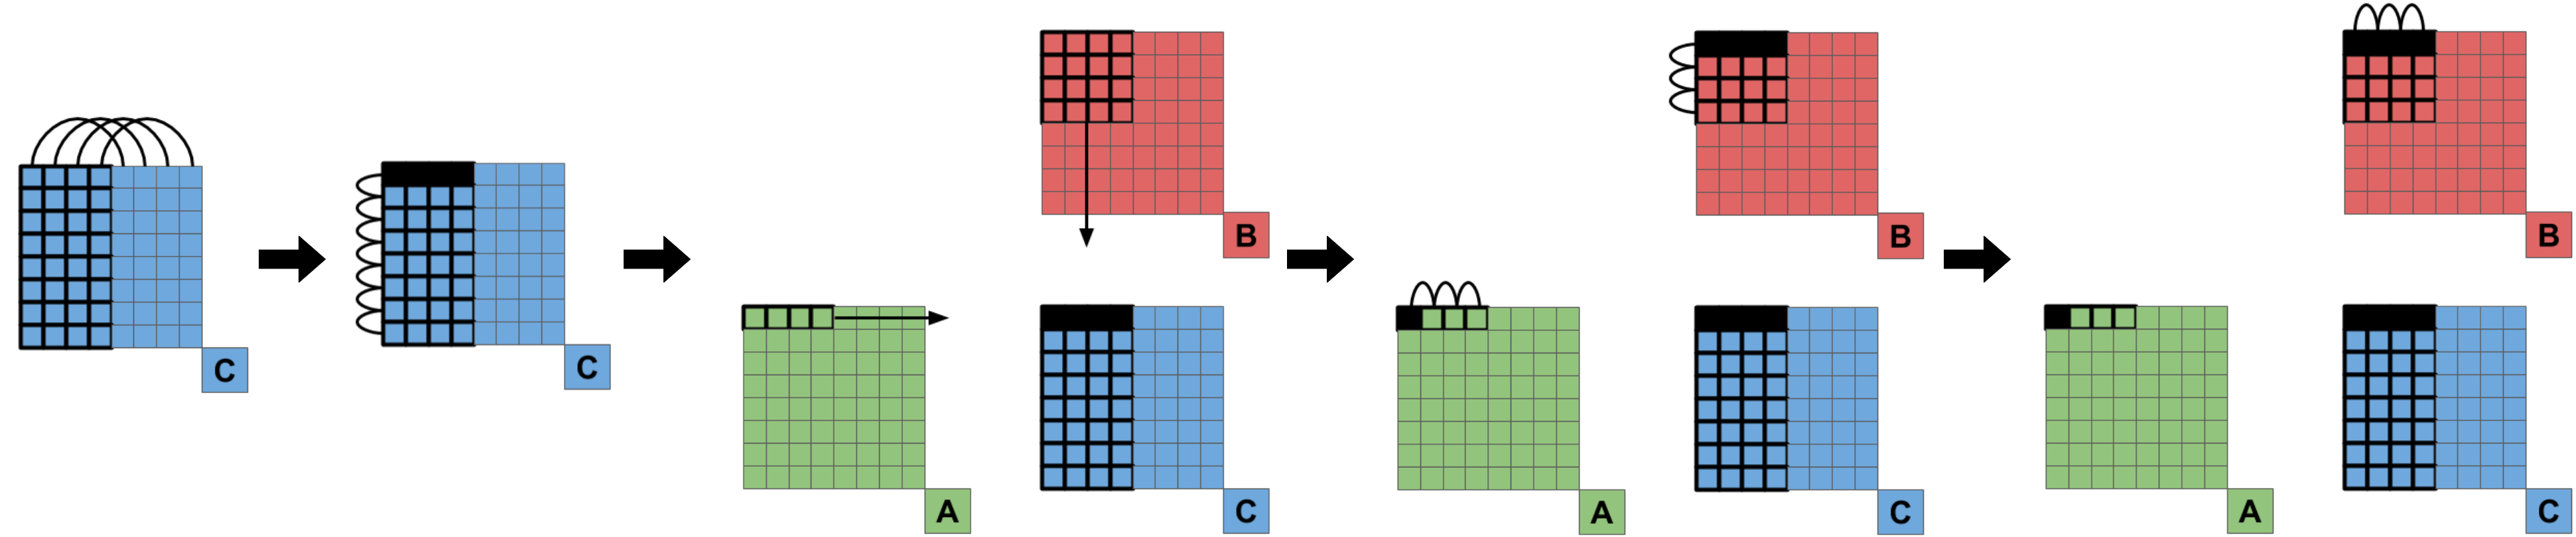
\includegraphics[width=1\textwidth]{resources/blocked_icon2.png}
    \end{adjustbox}
\end{frame}

%---------------------CUDA------------------------------
\section{CUDA}

\begin{frame}{\secname}
    In questa sezione si parlerà dell'implementazione in cuda del prodotto matrice matrice. \\ 
    
    Verranno presentate 3 versioni del codice che mostrano degli upgrade basandosi su uno sfruttamento migliore delle risorse a disposizione. \\

    Verranno inoltre affrontati gli aspetti di:
    \begin{itemize}
        \item Gestione del numero di thread
        \item Gestione della shared memory
        \item Gestione dei conflitti tra bank e accessi coalizzati
    \end{itemize}
\end{frame}

\subsection{1 versione}
\begin{frame}{\secname \text{ }- \subsecname\ }
    \begin{columns}
        \column{0.5\textwidth}
            \begin{minipage}{1\textwidth}
                \begin{adjustbox}{margin=0cm 0cm 0cm 0cm, center} % left, bottom, right, top
                    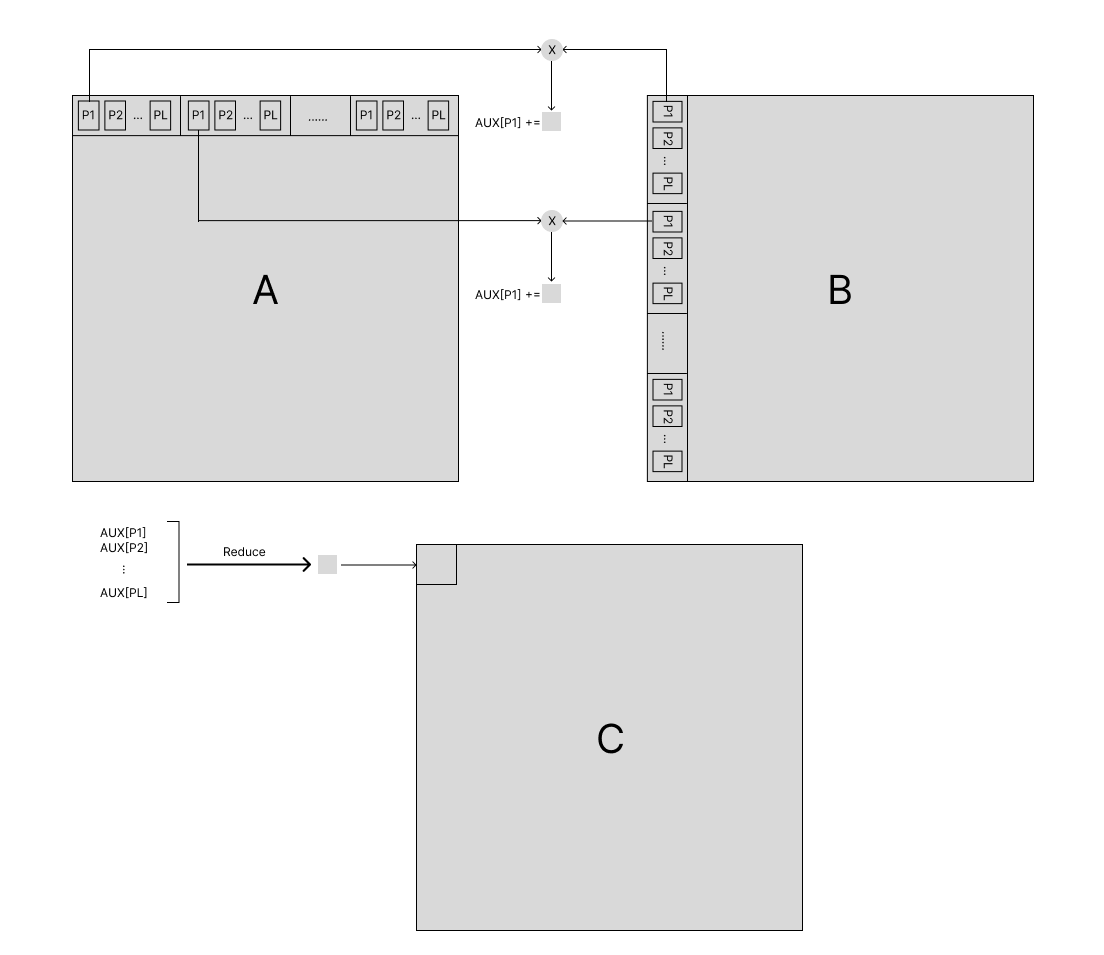
\includegraphics[width=1.2\textwidth]{resources/cuda_scheme_v1.png}
                \end{adjustbox}
            \end{minipage}
        \column{0.5\textwidth}
            \begin{minipage}[b]{1\textwidth}
                \begin{enumerate}
                    \item Divisione della riga di A tra i thread
                    \item Divisione della colonna di B tra i thread
                    \item Calcolo del prodotto per ogni thread
                    \item Memorizzazione dei risultati parziali in shared memory
                    \item Reduce dei risultati parziali
                    \item Scrittura sulla matrice C
                    \item Ripeti per ogni colonna di B
                    \item Ripeti per ogni riga di A
                \end{enumerate}
            \end{minipage}
    \end{columns}
\end{frame}

\begin{frame}{\secname \text{ }- \subsecname\ }
    Nella versione 1 tra il calcolo di una colonna e l'altra, i thread devono sincronizzarsi per poi fare l'operazione di reduce dei risultati parziali. \\ \\
    Questo perchè il vettore in shared memory riesce a contenere solo i risultati della riga di A per 1 colonna di B. \\
    
    \textbf{Soluzione:} \\
    Utilizzare una matrice di shared memory che mantiene i risultati parziali di più colonne per volta.
   \[
        aux = \left[
        \begin{matrix}
        pr_{col_0, t_0} & pr_{col_0, t_2} & ... & pr_{col_0, t_{BD}} \\
        pr_{col_1, t_0} & pr_{col_1, t_2} & ... & pr_{col_1, t_{BD}} \\
        ... & ... & ... & ... \\
        pr_{col_{Q}, t_0} & pr_{col_{Q}, t_2} & ... & pr_{col_{Q}, t_{BD}}
        \end{matrix}\right]
    \]
\end{frame}

\subsection{2 versione}
\begin{frame}{\secname \text{ }- \subsecname\ }
    \begin{columns}
        \column{0.5\textwidth}
        \begin{minipage}[b]{1\textwidth}
            \begin{enumerate}
                \item Divisione della riga di A tra i thread
                \item Divisione delle colonna di B \\tra i thread
                \item Calcolo del prodotto per ogni thread per tutto il gruppo di colonne
                \item Memorizzazione dei risultati parziali in shared memory
                \item Reduce dei risultati parziali 
                \item Scrittura sulla matrice C
                \item Ripeti per ogni gruppo di colonne di B
                \item Ripeti per ogni riga di A
            \end{enumerate}
        \end{minipage}
        \column{0.5\textwidth}
        \begin{minipage}{1.25\textwidth}
            \begin{adjustbox}{margin=0cm 0cm 0cm 0cm, center} % left, bottom, right, top
                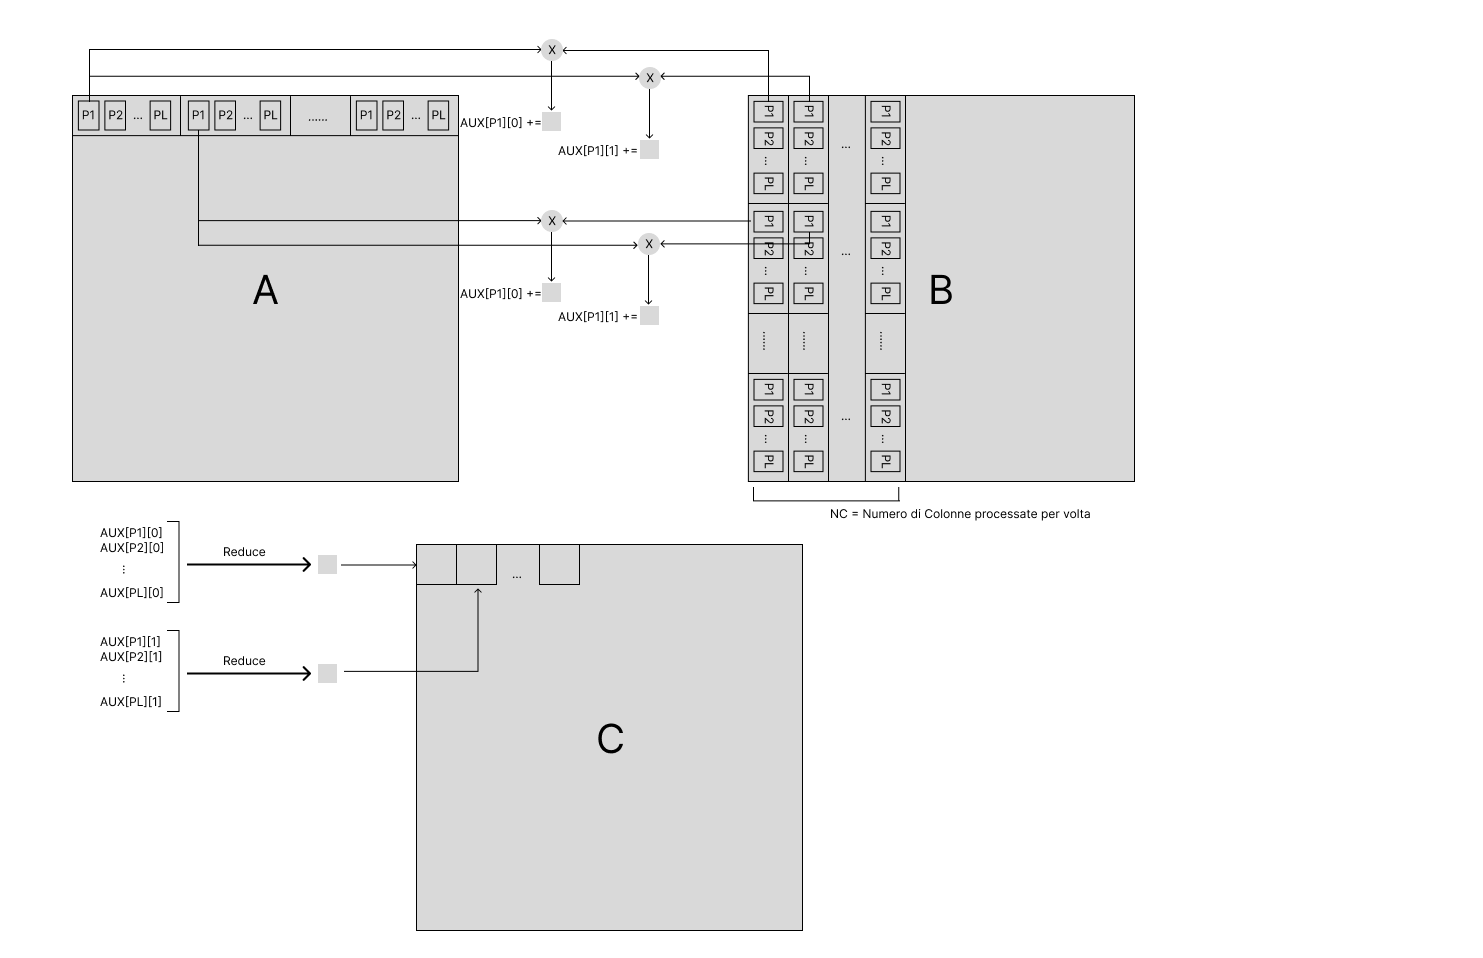
\includegraphics[width=1.2\textwidth]{resources/cuda_scheme_v2.png}
            \end{adjustbox}
        \end{minipage}
        
    \end{columns}
\end{frame}

\begin{frame}{\secname \text{ }- \subsecname\ }
    Nella versione 2 quando si processa il gruppo di colonne, poiché si calcola il risultato parziale di una colonna per volta, per ognuna di esse bisogna riaccedere alla riga della matrice A che è in memoria globale. \\ \\
    
    \textbf{Soluzioni:} \\
    \begin{itemize}
        \item Anziché processare una colonna per volta si processano i primi $BD$ elementi delle Q colonne del gruppo corrente.
        \begin{itemize}
            \item Questo permette di accedere una sola volta alla riga di A.
        \end{itemize}
        \item Mantenere in shared memory parte della colonna A necessario per il calcolo.
        \begin{itemize}
            \item Questo permette di accedere alla memoria globale una sola volta.
            \item Ogni thread accede al proprio elemento della riga di A necessario per il calcolo dalla memoria shared.
        \end{itemize}
    \end{itemize}
\end{frame}

\subsection{3 versione}

\begin{frame}{\secname \text{ }- \subsecname\ }
    \begin{columns}
        \column{0.5\textwidth}
        \begin{minipage}[b]{1\textwidth}
            \begin{enumerate}
                \item Divisione della riga di A tra i thread
                \item Divisione delle colonna di B \\ tra i thread
                \item Memorizzazione della riga parziale di A in shared memory
                \item Calcolo del prodotto per ogni thread per il blocco di righe \\ del gruppo di colonne 
                \begin{itemize}
                    \item ripeti per ogni blocco di \\ righe del gruppo di colonne
                \end{itemize}
                \item Memorizzazione dei risultati parziali in shared memory
                \item Reduce dei risultati parziali 
                \item Scrittura sulla matrice C
                \item Ripeti per ogni gruppo di colonne di B
                \item Ripeti per ogni riga di A
            \end{enumerate}
        \end{minipage}
        \column{0.5\textwidth}
        \begin{minipage}{1.25\textwidth}
            \begin{adjustbox}{margin=0cm 1cm 0cm 0cm, center} % left, bottom, right, top
                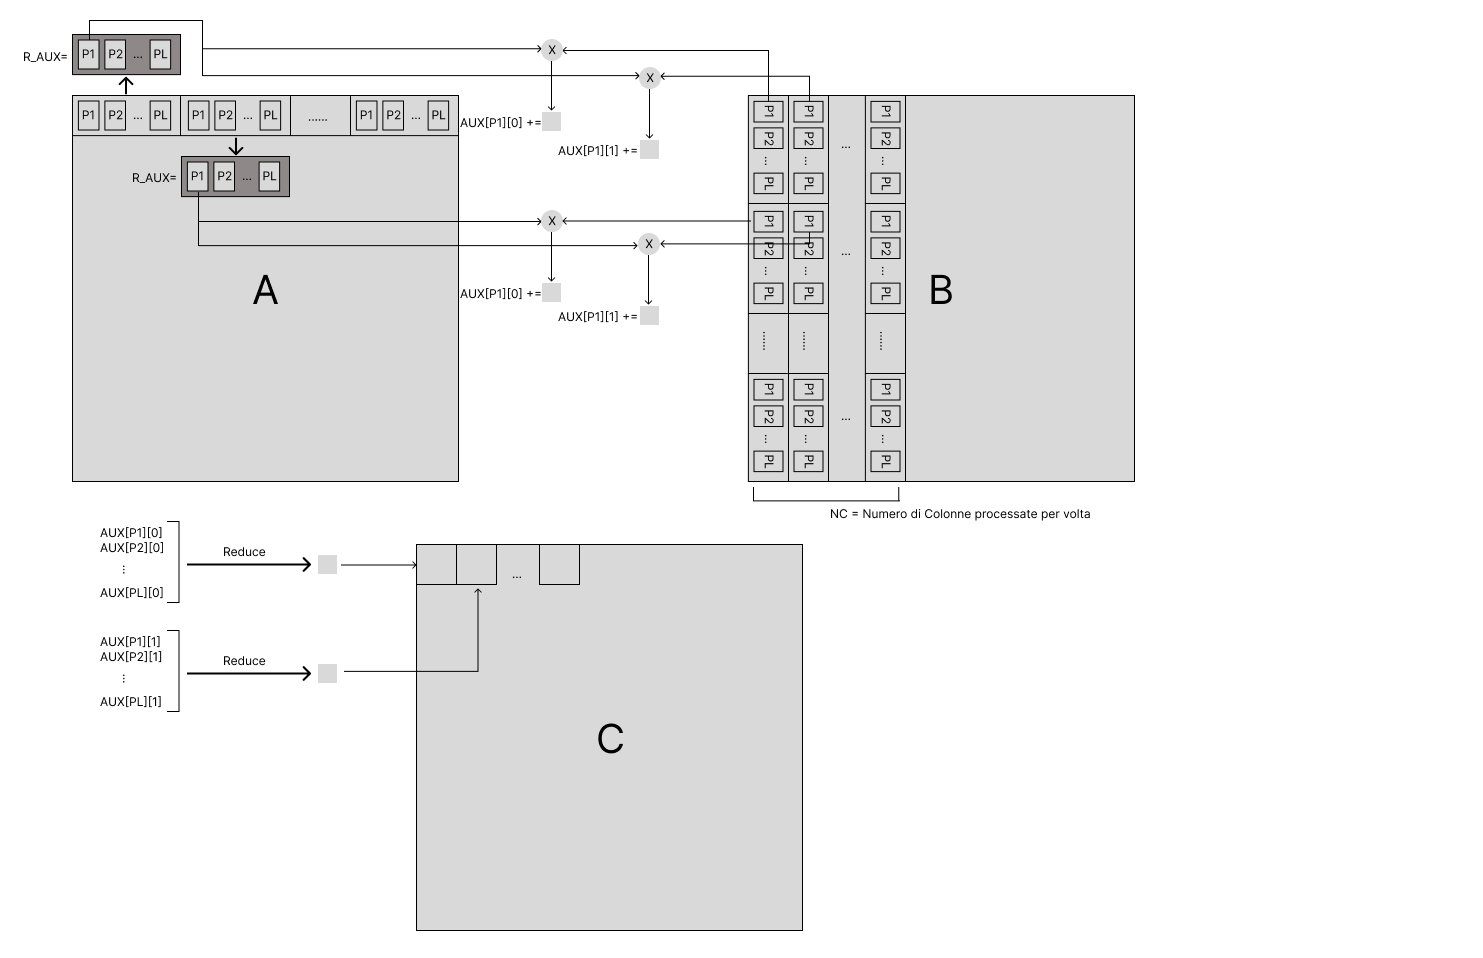
\includegraphics[width=1.1\textwidth]{resources/cuda_scheme_v3.png}
            \end{adjustbox}
        \end{minipage}
        
    \end{columns}
\end{frame}
\subsection{Configurazione dei parametri}
\subsubsection*{Thread}
\begin{frame}{\secname \text{ }- \subsecname\ \text{ }- \subsubsecname}
    \begin{itemize}
        \item Griglia unidimensionale di dimensione pari al numero di righe della matrice A
        \begin{itemize}
            \item Dovuto al fatto che ogni blocco è responsabile di una singola riga della matrice A
        \end{itemize}
        \item Numero di thread per ogni blocco (block size) pari a 256.
        \begin{itemize}
            \item Difficile stabilire un valore ottimale
            \item Si è rivelato il più efficiente in termini di prestazioni
            \item Multiplo di 32, dimensione del warp
        \end{itemize}
    \end{itemize}
    \begin{minipage}{0.4\textwidth}
        \centering
        \begin{adjustbox}{margin=6cm 0.3cm 0cm 0.3cm, center} % left, bottom, right, top
            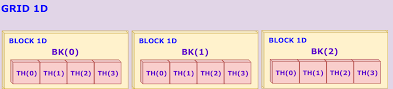
\includegraphics[width=1.1\textwidth, frame]{resources/grid1d.png}
        \end{adjustbox}
    \end{minipage}
\end{frame}

\subsubsection*{Shared memory}
\begin{frame}{\secname \text{ }- \subsecname\ \text{ }- \subsubsecname}
    \begin{itemize}
        \item 1 versione:
        \begin{itemize}
            \item \(size = BD \cdot 4\)
        \end{itemize}
        \item 2 versione:
        \begin{itemize}
            \item \(size = BD \cdot NC \cdot 4\)
        \end{itemize}
        \item 3 versione:
        \begin{itemize}
            \item \(size = (BD \cdot NC + BD) \cdot 4 = 4 (BD \cdot (NC + 1))\)
        \end{itemize}
    \end{itemize}
    \vspace{0.5cm}
    Avrebbe senso scegliere un valore di \(NC\) tale da massimizzare la shared memory disponibile, tuttavia tale approccio non porta a prestazioni migliori. \\ \\
    Quindi è stato utilizzato un approccio empirico per la scelta di \(NC\), scegliendo il valore con prestazioni maggiori, ovvero \(NC = 28\).
\end{frame}

\subsubsection*{Bank conflit}
\begin{frame}{\secname \text{ }- \subsecname\ \text{ }- \subsubsecname}
    Verrà analizzata solo la versione 3 perché tutti gli altri casi sono sottoinsiemi di questo.\\ \\
    2 possibili utilizzi della shared memory: 
    \begin{itemize}
        \item Memorizzare la riga della matrice A 
        \begin{itemize}
            \item Si memorizza un pezzo per volta di matrice A pari al numero di thread
            \item Ogni warp accede a 32 elementi contigui per volta
            \begin{itemize}
                \item pattern di accesso lineare con stride di una word da 32 bit
            \end{itemize}
        \end{itemize}
        \item Memorizzare il vettore dei risultati parziali
        \begin {itemize}
            \item Matrice aux row-order major
            \item Ogni warp accede a 32 elementi contigui per volta
            \begin{itemize}
                \item pattern di accesso lineare con stride di una word da 32 bit
            \end{itemize}
        \end{itemize}
    \end{itemize}
\end{frame}

%---------------------MPI+CUDA------------------------------
\section{MPI+CUDA}

\begin{frame}{\secname}
    %TODO
\end{frame}

%---------------------Analisi delle prestazioni------------------------------
\section{Analisi delle prestazioni}

\subsection{MPI}
\begin{frame}{\secname \text{ }- \subsecname\ }
    %TODO
\end{frame}

\subsubsection*{Matrici quadrate}
\begin{frame}{\secname \text{ }- \subsecname\ \text{ }- \subsubsecname}
    %TODO
\end{frame}

\subsubsection*{Matrici rettangolari}
\begin{frame}{\secname \text{ }- \subsecname\ \text{ }- \subsubsecname}
    %TODO
\end{frame}

\subsection{CUDA}
\subsubsection*{Matrici quadrate}
\begin{frame}{\secname \text{ }- \subsecname\ \text{ }- \subsubsecname}
    \begin{minipage}{0.85\textwidth}
        \centering
        \begin{adjustbox}{margin=2cm 0cm 0cm 0cm, center} % left, bottom, right, top
            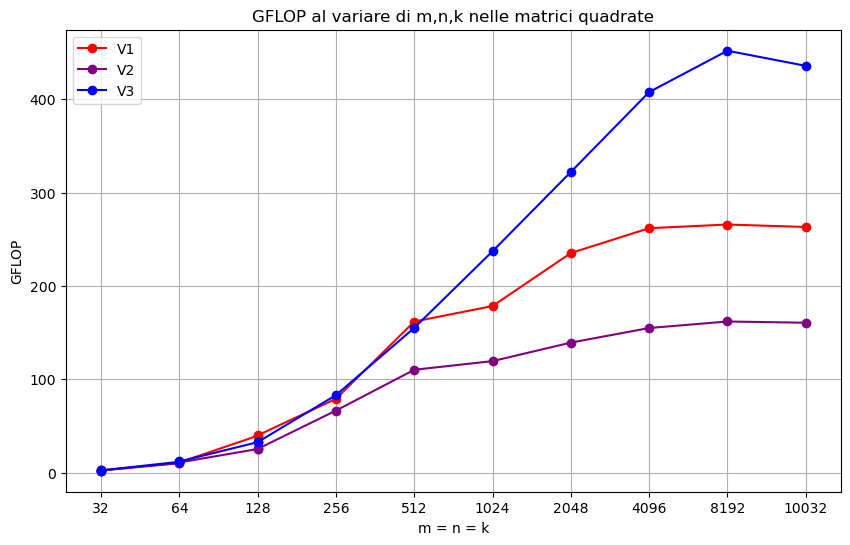
\includegraphics[width=1.1\textwidth, frame]{resources/gpu_matrix_square.png}
        \end{adjustbox}
    \end{minipage}
    
\end{frame}
\begin{frame}{\secname \text{ }- \subsecname\ \text{ }- \subsubsecname}
    \begin{itemize}
        \item V3 prestazioni migliori
        \begin{itemize}
            \item dovuto al fatto che essa sfrutta al meglio la shared memory e riduce il numero di accessi alla memoria globale
        \end{itemize}
        \item V2 prestazioni peggiori di V1
        \begin{itemize}
            \item Complessità aggiuntiva dovuta alla necessità di gestire un numero di colonne diverso da 1
            \item Potrebbe aver portato a ridurre i benefici introdotti e quindi ad ottenere delle prestazioni minori
        \end{itemize}
    \end{itemize}
    
\end{frame}



\subsubsection*{Matrici rettangolari}
\begin{frame}{\secname \text{ }- \subsecname\ \text{ }- \subsubsecname}
    \begin{columns}
        \column{0.5\textwidth}
            \begin{minipage}{0.8\textwidth}
                \centering
                \begin{adjustbox}{margin=1cm 0cm 0cm 0cm, center} % left, bottom, right, top
                    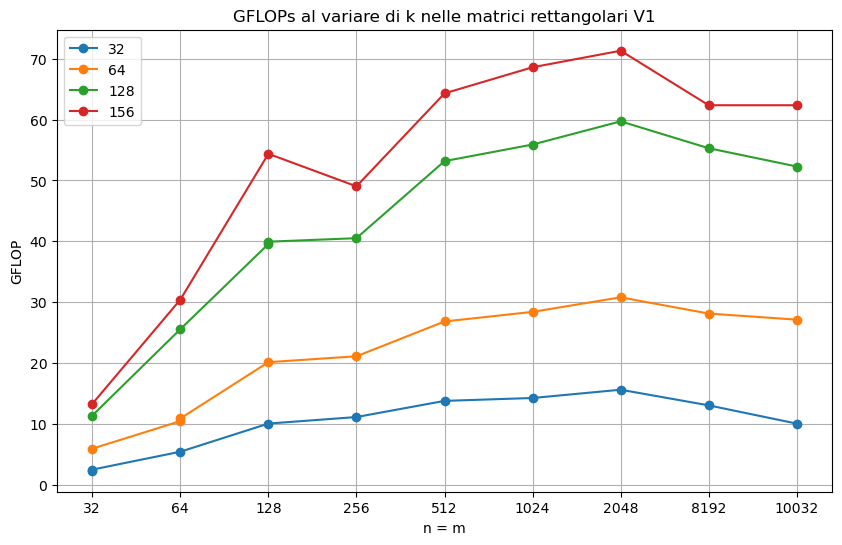
\includegraphics[width=1.1\textwidth, frame]{resources/gpu_matrix_rect_perfv1.png}
                \end{adjustbox}
            \end{minipage}
        \column{0.5\textwidth}
            \begin{minipage}{0.8\textwidth}
                \centering
                \begin{adjustbox}{margin=1.5cm 0cm 0cm 0cm, center} % left, bottom, right, top
                    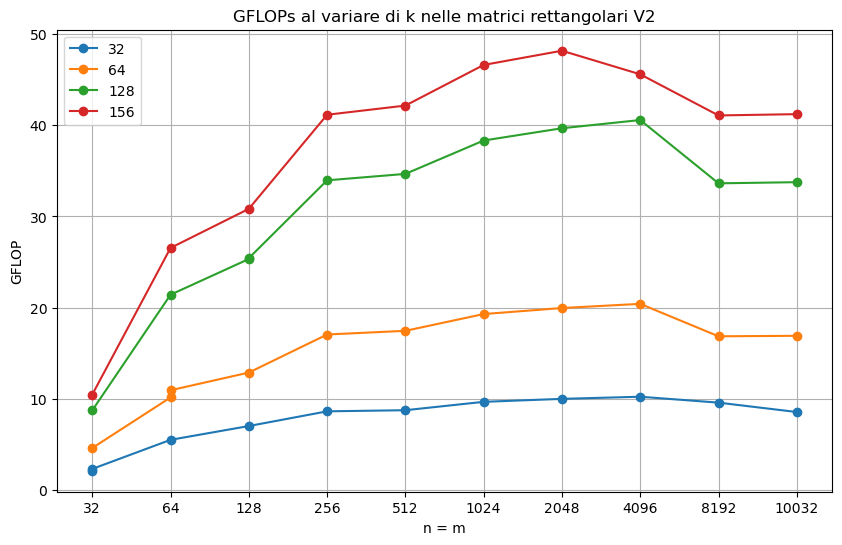
\includegraphics[width=1.1\textwidth, frame]{resources/gpu_matrix_rect_perfv2.png}
                \end{adjustbox}
            \end{minipage}
    \end{columns}
    \begin{minipage}{0.45\textwidth}
        \centering
        \begin{adjustbox}{margin=7cm 0cm 0cm 0.2cm, center} % left, bottom, right, top
            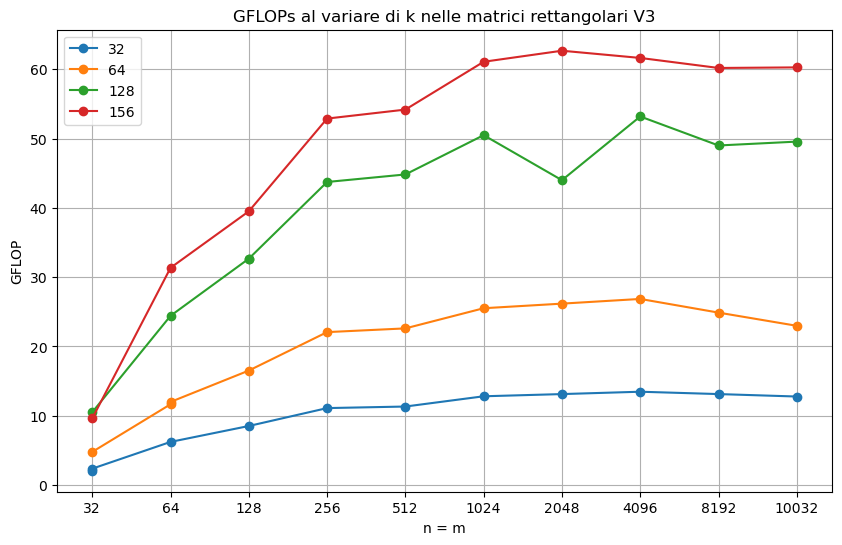
\includegraphics[width=1.1\textwidth, frame]{resources/gpu_matrix_rect_perfv3.png}
        \end{adjustbox}
    \end{minipage}
\end{frame}

\begin{frame}{\secname \text{ }- \subsecname\ \text{ }- \subsubsecname}
    \begin{itemize}
    \item Si può notare un calo considerevole delle prestazioni rispetto alla versione quadrata.
        \begin{itemize}
            \item ogni blocco lavora su una singola riga della colonna A alla volta, dividendola per il numero di thread in quel blocco
            \item ogni riga della matrice A è grande k, il quale è minore del numero di thread
            \item molti thread per ogni blocco che non fanno nulla, impatto dell'overhead di averli creati
            \item prestazioni peggiorano sempre più al diminuire del valore di k proprio perché il numero di thread inutili aumenta
        \end{itemize}

    \item Al contrario del caso quadrato non c'è un punto in cui c'è un calo delle prestazioni dovuto al trasferimento di memoria
        \begin{itemize}
            \item Matrici rettangolari sono più piccole $\Rightarrow$ tempo di trasferimento è minore 
            \item non si arriva al punto di annullare la controparte di calcolo
        \end{itemize}
    \end{itemize} 
\end{frame}

\subsection{MPI+CUDA}
\begin{frame}{\secname \text{ }- \subsecname\ }
    Limiti intrinsechi:
    \begin{itemize}
        \item Nel server dove sono stati fatti gli esperimenti è presente una sola GPU
        \begin{itemize}
            \item limitazione notevole dato che il vantaggio di utilizzare la soluzione MPI+CUDA è proprio quello di poter utilizzare le GPU di più server
            \item quando i processi andranno a tentare di eseguire concorrentemente il nucleo di calcolo su CPU, essi verranno serializzati
            \item Sfruttamento limitato del potenziale della soluzione
        \end{itemize}
        \item Le prestazioni calcolate contengono anche il conteggio del trasferimento della memoria RAM alla memoria globale della GPU
        \begin{itemize}
            \item non confrontabili direttamente con le prestazioni ottenute con la soluzione solo CUDA
        \end{itemize}
    \end{itemize}
\end{frame}

\subsubsection*{Matrici quadrate}
\begin{frame}{\secname \text{ }- \subsecname\ \text{ }- \subsubsecname}
    \begin{columns}
        \column{0.5\textwidth}
            \begin{itemize}
                \item - Processi $\Rightarrow$ + Performance
                \item Overhead memoria con \\matrici grandi
            \end{itemize}
        \column{0.6\textwidth}
            \begin{minipage}{0.85\textwidth}
                \centering
                \begin{adjustbox}{margin=0cm 0cm 0cm 0cm, center} % left, bottom, right, top
                    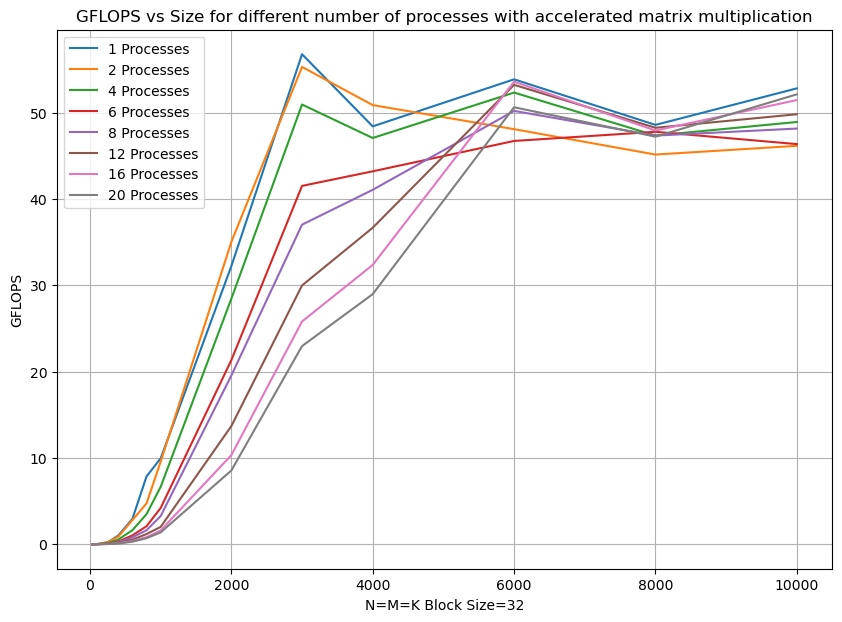
\includegraphics[width=1.1\textwidth, frame]{resources/mpi_cuda_square.png}
                \end{adjustbox}
            \end{minipage}
    \end{columns}
\end{frame}

\subsubsection*{Matrici rettangolari}
\begin{frame}{\secname \text{ }- \subsecname\ \text{ }- \subsubsecname}
    \begin{columns}
        \column{0.5\textwidth}
            \begin{minipage}{0.75\textwidth}
                \centering
                \begin{adjustbox}{margin=2cm 0cm 0cm 0cm, center} % left, bottom, right, top
                    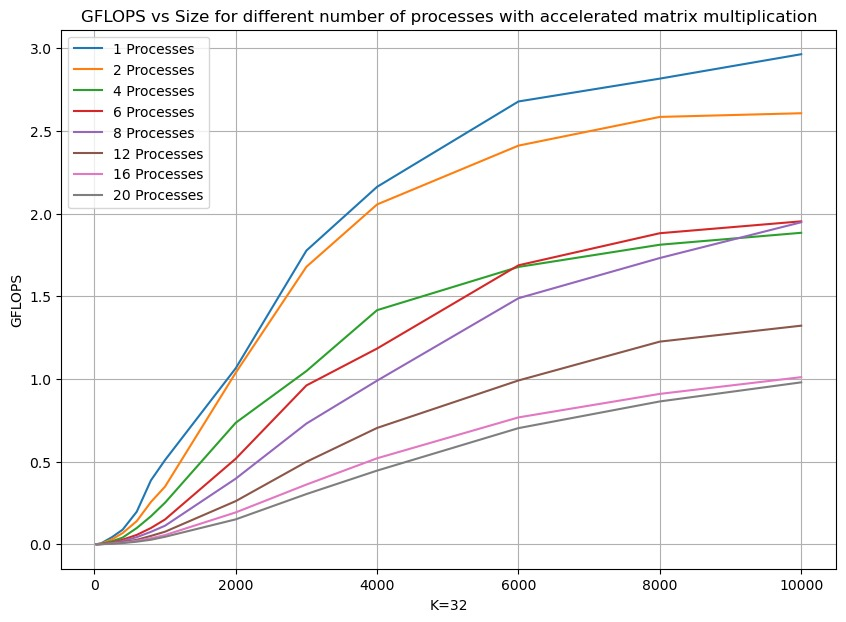
\includegraphics[width=1.1\textwidth, frame]{resources/mpi_cuda_32.jpg}
                \end{adjustbox}
            \end{minipage}
        \column{0.5\textwidth}
            \begin{minipage}{0.75\textwidth}
                \centering
                \begin{adjustbox}{margin=1cm 0cm 0cm 0cm, center} % left, bottom, right, top
                    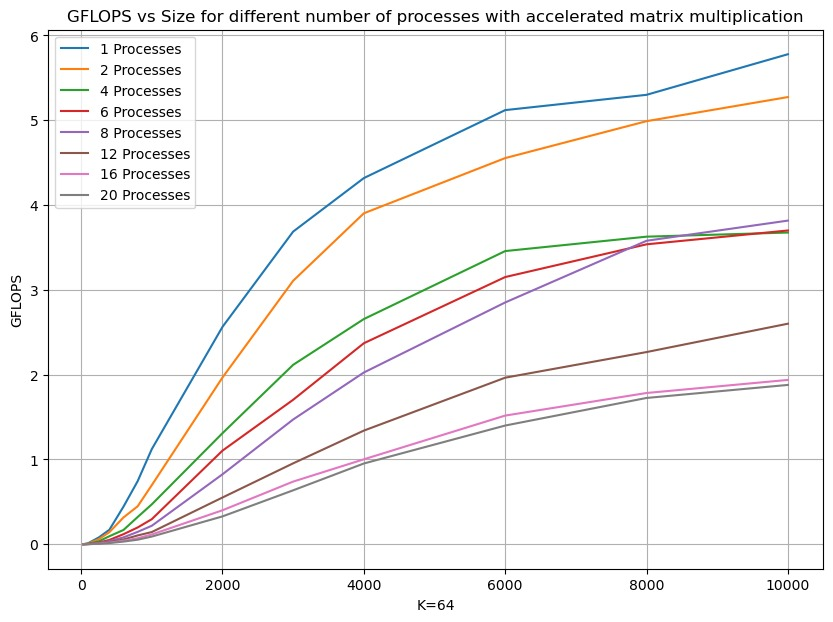
\includegraphics[width=1.1\textwidth, frame]{resources/mpi_cuda_64.jpg}
                \end{adjustbox}
            \end{minipage}
    \end{columns}
    \begin{columns}
        \column{0.5\textwidth}
            \begin{minipage}{0.75\textwidth}
                \centering
                \begin{adjustbox}{margin=2cm 0cm 0cm 0cm, center} % left, bottom, right, top
                    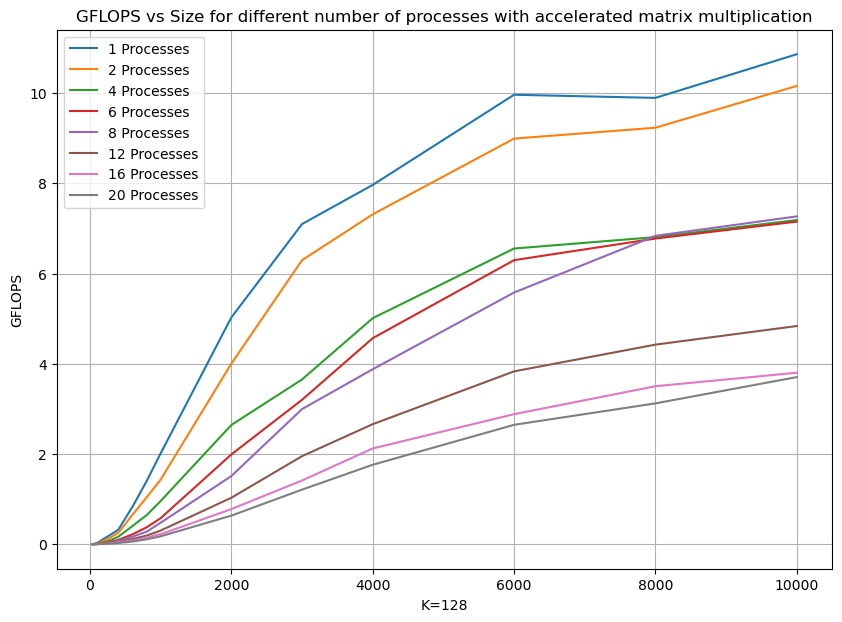
\includegraphics[width=1.1\textwidth, frame]{resources/mpi_cuda_128.jpg}
                \end{adjustbox}
            \end{minipage}
        \column{0.5\textwidth}
            \begin{minipage}{0.75\textwidth}
                \centering
                \begin{adjustbox}{margin=1cm 0cm 0cm 0cm, center} % left, bottom, right, top
                    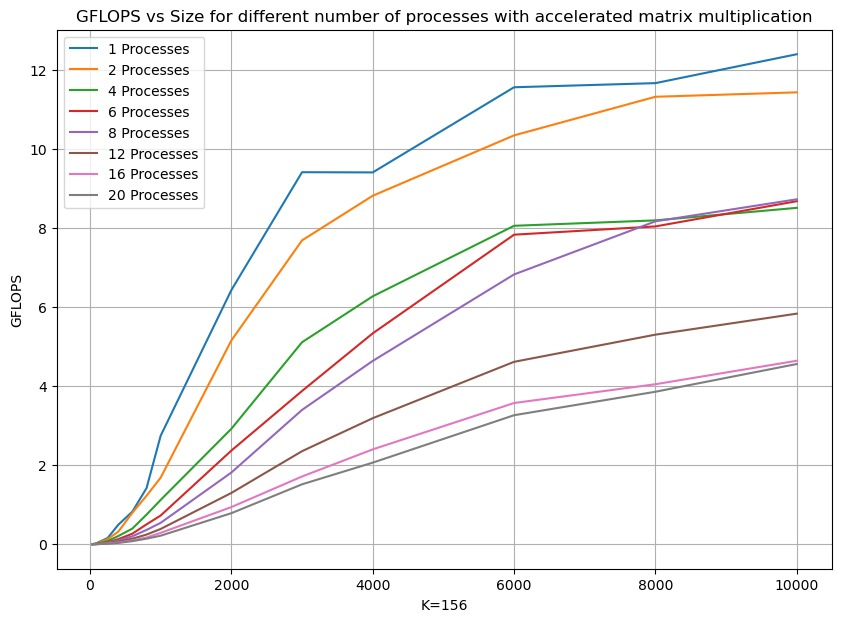
\includegraphics[width=1.1\textwidth, frame]{resources/mpi_cuda_156.jpg}
                \end{adjustbox}
            \end{minipage}
    \end{columns}
\end{frame}

\begin{frame}{\secname \text{ }- \subsecname\ \text{ }- \subsubsecname}
    \begin{itemize}
        \item Trend leggermente diverso nel quale al diminuire di k le prestazioni migliorano al contrario di quello che succedeva con il solo codice CUDA
        \begin{itemize}
            \item trasferimento di memoria nel calcolo esso sia un fattore determinante che aiuta matrici più piccole a ottenere prestazioni migliori
        \end{itemize}
        \item Al contrario del caso quadrato non c'è un punto in cui c'è un calo delle prestazioni dovuto al trasferimento di memoria
        \begin{itemize}
            \item Probabilmente dovuto al fatto che le matrici rettangolari sono più piccole e quindi il tempo di trasferimento è minore e non si arriva al punto di annullare la controparte di calcolo.
        \end{itemize} 
    \end{itemize}
\end{frame}




\begin{frame}
    \frametitle{Grazie per l'attenzione!}
    \begin{itemize}
        \item Tutto il codice che implementa il progetto è disponibile al
        seguente repository: \href{https://github.com/LucaFalasca/ParallelMatrixMultiplication}{https://github.com/LucaFalasca/ParallelMatrixMultiplication}
        \item contattaci a:
            \begin{itemize}
                \item \href{mailto:matteo.conti@students.uniroma2.eu}{matteo.conti@students.uniroma2.eu}
                \item \href{mailto:luca.falasca@students.uniroma2.eu}{luca.falasca@students.uniroma2.eu}
            \end{itemize}
       \end{itemize}
\end{frame}


\end{document}
